\documentclass[12pt,a4paper]{scrartcl}
\usepackage[utf8]{inputenc}
%\usepackage[latin1]{inputenc} %  Alternativ unter Windows
\usepackage[T1]{fontenc}
\usepackage[paper=a4paper,
left=25mm,
right=25mm,
top=25mm,
bottom=20mm]{geometry}
\usepackage[nottoc]{tocbibind}
\usepackage[ngerman]{babel}
\usepackage[pdftex]{graphicx}
\usepackage{latexsym}
\usepackage{amsmath,amssymb,amsthm,amsfonts}
\usepackage{mathtools}
\usepackage{enumitem}
\usepackage[utf8]{inputenc}
\usepackage{float}
\usepackage{physics}
\usepackage{subfigure}
\newcommand{\R}{\mathbb{R}}


\DeclareMathOperator{\dive}{div}
\newtheorem{Satz}{Satz}[section]\newtheorem{Definition}[Satz]{Definition} 
\newtheorem{Lemma}{Lemma}		                 
\newtheorem{Korollar}[Satz]{Korollar}
\newtheorem{Proposition}[Satz]{Proposition}                  
\newtheorem{examples}[Satz]{Beispiel}
\let\oldexamples\examples
\renewcommand{\examples}{\oldexamples\normalfont}
\newtheorem*{notation}{Notation}
\let\oldnotation\notation
\renewcommand{\notation}{\oldnotation\normalfont}
\newtheorem*{remark}{Bemerkung}
\let\oldremark\remark
\renewcommand{\remark}{\oldremark\normalfont}                  
\newtheorem*{define}{Definition}
\let\olddefine\define
\renewcommand{\define}{\olddefine\normalfont}

\usepackage{bbm}
\usepackage[german=quotes]{csquotes}
\usepackage{xcolor}
\newcommand*\diff{\mathop{}\!\mathrm{d}}
\DeclareMathOperator{\conv}{conv}
\DeclareMathOperator{\spann}{span}
\DeclareMathOperator{\Jacobi}{D}
\DeclareMathOperator{\diam}{diam}
\DeclareMathOperator{\hFgFE}{(hF gFE)}
\DeclareMathOperator{\dgFE}{(dgFE)}
\definecolor{Mygreen}{RGB}{0,128,0}
\newcommand{\defi}[1]{\textcolor{Mygreen}{#1}}
%\renewcommand{\phi}{\varphi}
\renewcommand{\epsilon}{\varepsilon}
\newcommand{\unklar}[1]{\textcolor{blue}{#1}}
\newcommand\restr[2]{{% we make the whole thing an ordinary symbol
		\left.\kern-\nulldelimiterspace % automatically resize the bar with \right
		#1 % the function
		\vphantom{\big|} % pretend it's a little taller at normal size
		\right|_{#2} % this is the delimiter
}}
\newcommand{\cupdot}{\mathbin{\mathaccent\cdot\cup}}
\DeclareMathOperator{\sign}{sign}

\numberwithin{equation}{section} 


% Praktikumsbericht nummer setzen
\newcommand{\BerichtNR}{2}

\begin{document}
\begin{titlepage}
	
\includegraphics[scale=0.5]{kit-logo.jpg} 
	\begin{center} 
		\LARGE 
		\vspace*{2cm}
		\LARGE Praktikumsbericht \BerichtNR
		\vspace*{1.0cm}
		\hrule
		\vspace*{0.2cm}
		{\vspace{0.2cm} \huge Einführung in das Wissenschaftliche Rechnen}\vspace{0.5cm}
		\hrule
		\vspace*{2.5cm}
		\Large Stefan Karch \\
		Florian Döttling \\
		Tim Buchholz  \\
		\vspace*{1cm}
		20.05.2019 \\
		\vspace*{1.5cm}
		\vspace*{4.0cm}
		\Large Betreuung: Prof. Dr. Christian Wieners, Niklas Baumgarten \\[0.5cm]
		\Large Fakultät für Mathematik \\
		\Large Karlsruher Institut für Technologie
	\end{center}
\end{titlepage}

\tableofcontents

\section{Zusammenfassung: gemischten Finite Elemente}
% !TeX root = Bericht_main.tex

\subsection{Analytische Herleitung}

\textbf{Ziel:} Wir wollen das Problem nun in einer Weise diskretisieren, sodass die Flussbilanz automatisch erfüllt ist (somit Flux Loss = 0).

Die Flussbilanz ist für die numerische Lösung erfüllt, wenn gilt:
\[ \int_{\Gamma_\text{in}} q_h \cdot n \diff a = \int_{\Gamma_\text{out}} q_h \cdot n \diff a \]
Bezeichnungen:
\begin{itemize}
	\item $ \Gamma_\text{in} $ und $ \Gamma_\text{out} $ analog definiert zu Lemma (1.1) im Skript
	\item n als äußerer Normalenvektor
	\item (Bisher bei Finiten Elementen) $ q_h \coloneqq \kappa \nabla_h u_h$ wobei $ \nabla_h $ eine \enquote{passende} numerische Differentiation-Methode ist.
\end{itemize}

Um die Flussbilanz zu erfüllen, verwenden wir \defi{gemischte Finite Elemente}. Bei dieser Methode wird, im Gegensatz zu (linearen) Finiten Elementen, nicht nur $ u_h $ als numerische Approximation für $ u $ berechnet, sondern das Paar $ (u_h,q_h) $ als numerische Approximation an $ (u,q) $. Wie genau dies funktioniert, untersuchen wir im Folgenden:

Betrachten wir noch einmal unser eigentliches analytisches Problem (LG: Laplace-Gleichung) 
\begin{gather*}
 \text{Bestimme } u:\overline{\Omega} \to \R \text{ mit }\\	
	\text{(LG)}\begin{cases}
	\dive \kappa \nabla u &= 0 \text{ in } \Omega\\
	u &= u_D \text{ auf } \Gamma_D \\
	(\kappa\nabla u) \cdot n &= g_N \text{ auf } \Gamma_N \\
	\end{cases}
\end{gather*}
($ \kappa $ ist sym. pos. def.) und setzen den \defi{Fluss} zu 
\[ q :\equiv - \kappa \nabla u. \]
Dann können wir unser analytisches Problem umschreiben zu 
\begin{gather*}
	\text{Bestimme } u:\overline{\Omega} \to \R \text{ und } q: u:\overline{\Omega} \to \R \text{ mit } \\
		\text{(LG F)}\begin{cases}
		\dive q &= 0 \text{ in } \Omega\\
		- \kappa \nabla u &= q \text{ in } \Omega\\
		u &= u_D \text{ auf } \Gamma_D \\
		-q \cdot n &= g_N \text{ auf } \Gamma_N \\
		\end{cases}
\end{gather*} 
der \defi{Laplace-Gleichung mit Fluss}. Nun schauen wir uns, wie zuvor bei Finiten Elementen, die schwache Formulierung von (LG F) an.

%TODO
\textcolor{red}{HERLEITUNG ÜBERSICHTLICHER AUFSCHREIBEN!}

\begin{align*}
	\int_\Omega \dive(q)\, \Phi \diff x = 0 &\text{ für alle Testfunktionen } \Phi: \Omega \to \R \\
	\int_{\Omega} \kappa^{-1} (q + \kappa \nabla u) \cdot \Psi \diff x = 0 &\text{ für alle Testfunktionen } \Psi:\Omega \to \R^2 \ (\star)
\end{align*}
Wir wollen nun noch die Dirichlet-Randbedingung $ 	u = u_D \text{ auf } \Gamma_D $ mit in die schwache Formulierung einfließen lassen. Dazu verwenden wir den Satz von Gauß:
\[ \int_{\partial\Omega} (u\Psi) \cdot n \diff a \stackrel{\text{Gauß}}{=} \int_{\Omega} \dive(u\Psi) \diff x = \int_{\Omega} \nabla u \cdot \Psi \diff x + \int_{\Omega} u \dive(\Psi) \diff x \quad (\Psi:\Omega \to \R^2) \]

Die Neumann-Randbedingung $ (\kappa\nabla u) \cdot n = g_N \text{ auf } \Gamma_N $ wird durch die Wahl des Lösungs- bwz. Ansatzraumes erfüllt.
\bigskip

Zusammen mit 
\begin{align*}
	&&\int_{\partial\Omega} (u\Psi) \cdot n \diff a &= \int_{\Gamma_D} (u_D\Psi) \cdot n \diff a &&(\Psi:\Omega \to \R^2 \text{ mit } \Psi \cdot n = 0 \text{ auf } \Gamma_N ) \\
	&\text{ und }\\
	&&(\star) \iff \int_{\Omega} \nabla u \cdot \Psi \diff x &= - \int_{\Omega} (\kappa^{-1} q) \cdot \Psi \diff x &&(\Psi:\Omega \to \R^2) 
\end{align*}
erhalten wir die gewünschte schwache Formulierung, im Folgenden \defi{gemischtes Finite-Elemente-Problem} genannt:
\begin{gather*}
	\text{Bestimme } (q,u) \text{ mit } q\cdot n = -g_N \text{ auf } \Gamma_N \text{ und}\\
	\text{(gFE)}\begin{cases}
		\int_{\Omega} \kappa^{-1} q \cdot \Psi \diff x \, - \mkern-15mu &\int_{\Omega} u \, \dive(\Psi) \diff x = - \int_{\Gamma_D} (u_D \Psi) \cdot n \diff a\\
		&\int_{\Omega} \dive(q) \, \Phi \diff x = 0
	\end{cases}	\\
	\text{ für alle } (\Psi, \Phi) \text{ mit } \Psi \cdot n = 0 \text{ auf } \Gamma_N 
\end{gather*}
\textbf{Idee der gemischten Finiten Elemente}: Diskretisieren wir (gFE), so erfüllt unsere numerische Lösung $ q_h $ die Forderung $ \dive(q_h) = 0 \text{ auf } K \ (K \in \mathcal{K}) $ und somit auch die Flussbilanz in jeder Zelle.

\subsection{Diskretisierung}

Sei $ \mathcal{K} $ eine zulässige Triangulierung von $ \Omega $ ($ \Omega = \bigcup_{K \in \mathcal{K}} K $).

Weiter sei $ \mathcal{F} $ die \defi{Menge aller Seiten}, $ \mathcal{F}_K $ die \defi{Menge aller Seiten von $ K $} und $ \partial \Omega_h $ der \defi{Rand von $ \Omega_h $}, formal definiert mit
\begin{align*}
	\mathcal{F} &\coloneqq \left( \{ \partial K_1 \cap \partial K_2 : K_1,K_2 \in \mathcal{K} \} \cup \{ \partial K_1 \cap \partial \Omega : K_1 \in \mathcal{K}\} \right) \setminus \{ \emptyset \} \\
	\mathcal{F}_K &\coloneqq \left( \{ \partial K \cap \partial K' : K' \in \mathcal{K} \} \cup \{ \partial K \cap \partial \Omega\} \right) \setminus \{ \emptyset \} \\
	\partial \Omega_h &\coloneqq \bigcup_{F \in \mathcal{F}} F.
\end{align*}
Wir nummerieren Seiten und Zellen durch:
\begin{align*}
	\mathcal{F} &= \{F_1, \dots , F_{\abs{\mathcal{F}}} \} &\text{\defi{globale Seitennummerierung}} \\
	\mathcal{K} &= \{K_1, \dots , K_{\abs{\mathcal{K}}} \} &\text{\defi{globale Zellennummerierung}} 
\end{align*}
\begin{remark}
	\begin{gather*}
	\text{Es gilt }\Omega = \Omega_h \cupdot \partial_h\Omega \cupdot \mathcal{V}_h. \\
	\Omega_h = \bigcup_{K \in \mathcal{K}} K \text{ (Flächen/Zellen)}\quad \partial_h\Omega = \bigcup_{F \in \mathcal{F}} F \text{ (Seiten)}\quad \mathcal{V}_h = \bigcup_{z \in \mathcal{V}}\{ z \} \text{ (Knoten)}	
	\end{gather*}
\end{remark}
\begin{define}
	Als Testräume/FE-Räume wählen wir $ W_h, Q_h $ und $ W_h(-g_N) $
	\begin{align*}
		W_h &\coloneqq \spann \left\{ \psi_1, \dots , \psi_{\abs{\mathcal{F}}}  \right\} &&\text{(\defi{Seitenansatzraum}/ Raum für $ \psi $ und $ q_u!!! $ mit RWen)}\\
		Q_h &\coloneqq \spann \{ \mu_1, \dots , \mu_{\abs{\mathcal{K}}} \} &&\text{(\defi{Zellenansatzraum}/ Raum für $ \phi $ und $ u_h $)}
	\end{align*}
	\begin{align*}
		W_h(g) &\coloneqq \left\{ \psi_h \in W_h: \int_F \psi_h \cdot \diff a = \int_F g \diff a \quad (F \subseteq \Gamma_N) \right\}.
	\end{align*}
	$ \{ \psi_i \}_{i=1}^{\abs{\mathcal{F}}} $ heißt \defi{Seitenbasis} und ist gegeben durch 
	\begin{align*}
		\forall i \in \{1, \dots , \abs{\mathcal{F}} \} : \int_{F_j} \psi_i \cdot n \diff a = \delta_{i,j} \text{ und }  \psi_i|_K \in \mathbb{P}_1(K,\R^2) \ (K \in \mathcal{K}) 
	\end{align*}
	und  $ \{ \mu_i \}_{m=1}^{\abs{\mathcal{K}}} $ heißt \defi{Zellenbasis} und ist gegeben durch
	\begin{align*}
		\forall m \in \{1, \dots , \abs{\mathcal{K}} \} : \mu_m \coloneqq  \mathbbm{1}_{K_m}.
	\end{align*}
\end{define}

\begin{remark}
	
	\[	\forall K \in \mathcal{K}:\psi_i|_K \in \mathbb{P}_1(K,\R^2) \text{ und } \mu_m|_K \in \mathbb{P}_0(K,\R) \]
	Unter Verwendung der Notation 
	\[\forall k,n \in  \mathbb{N} \ \forall K \in \mathcal{K}: \tilde{\mathbb{P}}_k(K,\R^n) \coloneqq \left\{  f:\Omega \to \R^n \mid f|_K \in \mathbb{P}_k(K, \R^n)  \right\}  \]
	gilt
	\begin{align*}	
	W_h &\subseteq \bigcap_{K \in \mathcal{K}} \tilde{\mathbb{P}}_1(K,\R^2) &&\text{(Menge der zellenweisen linearen Funktionen) und }\\
	Q_h &\subseteq \bigcap_{K \in \mathcal{K}} \tilde{\mathbb{P}}_0(K,\R) &&\text{(Menge der zellenweisen konstanten Funktionen)}. 
	\end{align*}	
\end{remark}

\begin{define}
	Weiter definieren wir das \defi{diskrete gemischte Finite-Elemente-Problem}:
	\begin{gather*}
		\text{Bestimme } (q_h,u_h) \in W_h(-g_N) \times Q_h \text{ mit}\\
		\dgFE\begin{cases}
			\int_{\Omega} \kappa ^{-1} q_h \cdot \psi_h \diff x \mkern-15mu &- \int_{\Omega} u_h \dive(\psi_h) \diff x = - \int_{\Gamma_D} u_D \psi_h \cdot n \diff a\\
			&- \int_{\Omega} \dive(q_h) \phi_h \diff x = 0
		\end{cases} \\
		\text{für alle } (\psi_h, \phi_h) \in W_h(0) \times Q_h
	\end{gather*}
\end{define}
\subsubsection{Referenzzelle}

Es bleibt die Frage offen, wie wir die Seitenbasis $ \{ \psi_i \}_{i=1}^{\abs{\mathcal{F}}} $ erhalten. Dazu betrachten wir, wie im Abschnitt zu Finiten Elementen, die Referenzzelle. Im Folgenden werden wir das Referenzdreieck anschauen, analog können die Schritte für das Referenzviereck vollzogen werden. 

\begin{define}
	
	Das \defi{Referenzdreieck} $ \triangle $ ist definiert als
	 \[ \hat{K} \coloneqq \conv \{ \hat{\mathcal{V}} \} \text{, wobei } \hat{\mathcal{V}} \coloneqq \left\{ 
	 \begin{pmatrix}
		 0\\
		 0
	 \end{pmatrix},
	 \begin{pmatrix}
		 1\\
		 0
	 \end{pmatrix},
	 \begin{pmatrix}
		 0\\
		 1
	 \end{pmatrix} \right\} \]
	Die Seiten des Referenzdreiecks sind
	\begin{align*}
	 	\hat{F}_0 &\coloneqq \conv \left\{ 
	 	\begin{pmatrix}
	 		0\\
	 		0
	 	\end{pmatrix},
	 	\begin{pmatrix}
		 	1\\
		 	0
	 	\end{pmatrix} \right\}\\
	 	\hat{F}_1 &\coloneqq \conv \left\{ 
	 	\begin{pmatrix}
		 	1\\
		 	0
	 	\end{pmatrix},
	 	\begin{pmatrix}
		 	0\\
		 	1
	 	\end{pmatrix} \right\}\\
	 	\hat{F}_2 &\coloneqq \conv \left\{ 
	 	\begin{pmatrix}
		 	0\\
		 	1
	 	\end{pmatrix},
	 	\begin{pmatrix}
		 	0\\
		 	0
	 	\end{pmatrix} \right\}\\ 	
	\end{align*}
	die Seitenbasis ist gegeben durch
	\begin{align*}
	 	\hat{\psi}_0:\hat{K} \to \R^2, \hat{\psi}_0(\xi) &\coloneqq 
	 	\begin{pmatrix}
	 		\xi_1\\
	 		\xi_2-1
	 	\end{pmatrix}\\
	 	\hat{\psi}_1:\hat{K} \to \R^2, \hat{\psi}_1(\xi) &\coloneqq  
	 	\begin{pmatrix}
		 	\xi_1\\
		 	\xi_2
	 	\end{pmatrix}\\
	 	\hat{\psi}_2:\hat{K} \to \R^2, \hat{\psi}_2(\xi) &\coloneqq 
	 	\begin{pmatrix}
		 	\xi_1-1\\
		 	\xi_2
	 	\end{pmatrix}.
	\end{align*}
	und $ \hat{n} $ sei der äußere Normalenvektor von $ \hat{K} $
\end{define}

\begin{remark}
 	$\forall i,j\in\{1,2,3\}: \int_{F_j} \hat{\psi}_i \cdot \hat{n} \diff a = \delta_{i,j} \text{ und } \hat{\psi}_i \in \mathbb{P}_1(\hat{K}, \R^2).$
\end{remark}

Weiter setzen wir noch 
\begin{align*}
\text{ die Menge der Seiten }&& \hat{\mathcal{F}} &\coloneqq \left\{ \hat{F}_0, \hat{F}_1, \hat{F}_2 \right\} \\
\text{und den Seitenansatzraum }&&  \hat{W} &\coloneqq \spann \left\{ \psi_0,\psi_1, \psi_2 \right\}.
\end{align*}
\textbf{Transformation von $ \hat{K} $ zu $ K $:} Für ein beliebiges $ K \in \mathcal{K} $ wollen wir jetzt eine Seitenbasis $ \{ \psi_1^K, \psi_2^K, \psi_3^K \} $ berechnen (Wie bisher gegeben durch $ \forall i\in\{1,2,3\}: \psi_i^K\in\mathbb{P}_1(K,\R^2) \text{ und } \int_{F_j^K} \psi_i^K \cdot n^K \diff a = \delta_{i,j} $, wobei $ n^K $ äußere Normale von  $ K $ und $ F_j^K  $ beliebige Seite von $ K $). Dazu betrachten wir die affine \defi{Transformationsabbildung $ \varphi_K $} von $ \hat{K} $ zu $ K $:
\begin{gather*}
	\varphi_K: \hat{K} \to K, \varphi_K(\xi) = z_{0,K} + B_K \xi \text{ mit passenden } B_K\in\R^{2 \times 2} \text{ und } \\
	J_K \coloneqq \det(B_K) > 0.
\end{gather*}
\begin{Lemma}
	Es gilt: $\tilde{n}^K = \frac{1}{\abs{B_K^{-T} \hat{n}}} B_K^{-T} \hat{n} $ ist Normale zu $ \partial K $.
\end{Lemma}
\begin{remark}
	\unklar{
	Damit $ \tilde{n}^K $ zu einer äußeren Normalen von $ K $ wird, betrachten wir für $ \hat{F} = \conv \{\hat{z}_j, \hat{z}_k\} $ als Seite von $ \hat{K} $ und $ F = \varphi_K(\hat{F}) = \conv \{ z_j , z_k \}$ als Seite von $ K = \varphi_K(\hat{K}) $:
	\begin{gather*}
		u_F \coloneqq\frac{1}{\abs{z_j-z_k}} 
		\begin{pmatrix}
			z_j[2] - z_k[2] \\
			z_k[1] - z_j[1]
		\end{pmatrix} \quad
		u_{\hat{F}} \coloneqq \frac{1}{\abs{\hat{z}_j-\hat{z}_k}} 
		\begin{pmatrix}
			\hat{z}_j[2] - \hat{z}_k[2] \\
			\hat{z}_k[1] - \hat{z}_j[1]
		\end{pmatrix} \\
		s_{K,F} \coloneqq \sign(u_F \cdot B_F^{-T} u_{\hat{F}}).
	\end{gather*} 
	Wir erhalten die äußere Normale durch 
	\[ n^K = s_{K,F} \; \tilde{n}^K \]
	}
\end{remark} 
Weiter bekommen wir unsere Seitenbasis auf $ K $ durch 
\[ \psi_i^K = J_K^{-1}B_K \hat{\psi}_i \circ \varphi_K \ (i\in \{1,2,3\}) \]
\begin{remark}
	Es gilt: $ \hat{\psi}_i \cdot \hat{n} = 0 \iff \psi_i^K \cdot n = 0 $
\end{remark}
Um  an unsere Seitenbasis auf $ \Omega \ \{\psi_j\}_{j = 1}^{\abs{\mathcal{F}}}$ zu kommen, benötigen wir noch die Übersetzung der globalen Seitennummerierung in einer Zelle $ K $ zur globalen Seitennummerierung
\[ l:\mathcal{K}\times \{1,2,3\} \to \{1, \dots , \abs{\mathcal{F}} \}, (K,i) \mapsto l(K,i). \]
Wir setzen $ \psi_j (j \in \{1,\dots , \abs{\mathcal{F}}\})$ durch
\[ \psi_j(x) = 
\begin{cases}
	\psi_i^K(x) , &\text{falls } j = l(K,i)\\
	0,			  &\text{sonst}.
\end{cases} \]
\begin{remark}
	Für alle Zellen $ K \in \mathcal{K} $ von denen $ F_j $ eine anliegende Seite ($ \overline{K} \cap F_j \ne \emptyset $) und $ F_j $ lokal mit $ i \in \{1,2,3\} $ nummeriert ist, gilt:
	\[ \psi_j|_K = \psi_i^K. \]
\end{remark}

\subsection{Formulierung als LGS}
Seien wie oben Seiten, Seitenbasis, Zellen und Zellenbasis global nummeriert 
\begin{align*}
&N \coloneqq \abs{\mathcal{F}} &&\mathcal{F} = \{F_1, \dots , F_{N} \}  \\
&&&W_h =\{\psi_1, \dots , \psi_N\}\\
&M \coloneqq \abs{\mathcal{K}} &&\mathcal{K} = \{K_1, \dots , K_{M} \}  \\
&&&Q_h = \{\mu_1 , \dots , \mu_M  \}.
\end{align*}

\begin{define}
	\begin{align*}
		&\underline{A} \in \R^{N \times N} \text{ mit } \underline{A}[n,k] \coloneqq \int_{\Omega} \kappa^{-1} \psi_n \cdot \psi_k \diff x \\
		&\underline{B} \in \R^{M \times N} \text{ mit } \underline{B}[m,k] \coloneqq - \int_{\Omega} \mu_m \dive(\psi_k) \diff x \\
		&\underline{b} \in \R^N \text{ mit } \underline{b}[k] \coloneqq - \int_{\Gamma_D} u_D \psi_k \cdot n \diff a
	\end{align*}
	und (für die Randbedingungen)
	\begin{gather*}
		\underline{W}(g) \coloneqq \left\{ \underline{q} \in \R^N : \underline{q}[k] = \int_{F_k} g  \diff a \ (\text{für } k \text{ mit} F_k \subseteq \Gamma_N) \right\} 
	\end{gather*}
\end{define}

\textbf{Umformung:} Unser zu lösendes Problem (dgFE) lässt sich mit $ q_h = \sum_{n=1}^{N} \underline{q}[n] \psi_n $ und $ u_h = \sum_{m=1}^{M} \underline{u}[m] \mu_m $ umformen zu 
\begin{gather*}
	\text{Bestimme} (\underline{q},\underline{u}) \in \underline{W}(-g_N)\times \R^M \text{ mit }\\
	\text{(L gFE)}\begin{cases}
		\underline{A} \underline{q} + \underline{B}^T \underline{u} &= \underline{b} \\
		\underline{B} \underline{q} &= 0
	\end{cases}
\end{gather*}
oder anders geschrieben 
\begin{gather*}
\text{Bestimme} (\underline{q},\underline{u}) \in \underline{W}(-g_N)\times \R^M \text{ mit }\\
	\text{(uL gFE)}\begin{cases}
		\begin{pmatrix}
			\underline{A} &\underline{B}^T\\
			\underline{B} &0
		\end{pmatrix}
		\begin{pmatrix}
			 \underline{q} \\
			 \underline{u} 
		\end{pmatrix}
		 =
		 \begin{pmatrix}
			 \underline{b}\\
			 0
		 \end{pmatrix}.
	\end{cases}
\end{gather*}

\subsection{Optimierungstheorie und Sattelpunktproblem}
\begin{Lemma}\label{Sattelpunkt} Sei $ (\underline{q},\underline{u}) \in \underline{W}(-g_N) \times \R^M $ und $ L $ gegeben durch 
\[L: \underline{W}(-g_N) \times \R^M \to \R, (\underline{x}, \underline{y}) \mapsto \frac{1}{2} \underline{x}^T \underline{A} \underline{x} - \underline{b}^T \underline{x} + \underline{y}^T \underline{B} \underline{x} \]
und es gilt: $ \forall (\underline{r}, \underline{v}) \in \underline{W}(-g_N) \times \R^M: L(\underline{q}, \underline{v}) \leq L(\underline{q}, \underline{u}) \leq L(\underline{r}, \underline{u}) $ (insb. ist $ (\underline{q},\underline{u}) $ ein Sattelpunkt von $ L $).

Dann löst $ (\underline{q}, \underline{u}) $ (L gFE) bzw. $ (q_h,u_h) $ (dgFE) (wobei $ q_h = \sum_{n=1}^N \underline{q}[n] \psi_n $ und $ u_h = \sum_{m=1}^M\underline{u}[m] \mu_m $).
\end{Lemma}

\textbf{Aus Optimierungstheorie:} 
\begin{gather*}
	(\underline{q}, \underline{u}) \text{ Sattelpunkt von } L  \text { wie in Lemma \ref{Sattelpunkt}}\\
	\iff \underline{q} \text{ minimiert } E:W_h(-g_N) \to \R , \underline{x} \mapsto \frac{1}{2} \underline{x}^T \underline{A} \underline{x} - \underline{b}^T \underline{x} \text{ unter der NB } \underline{B} \underline{q} = 0.
\end{gather*}

\begin{Satz}[Dual-Primal-Error] ~\newline
	Wir betrachten unser Ausgangsproblem \emph{(LG)} bzw. \emph{(LG F)}. Sei $ u_h \in V_h(u_D) $ Lösung des linearen FE-Verfahren (\defi{primale Lösung}) und $ q_h \in W_h(-g_N) $ Lösung des gemischten FE-Verfahren (\defi{duale Lösung}). 
	
	Dann gilt die A-posteriori Schranke (wobei  $ \norm{f}_{\kappa^{-1}} = \int \kappa^{-1} f \cdot f \diff x $ ) 
	\begin{gather*}
	\norm{q-q_h}_{\kappa^{-1}} \leq \underbrace{\norm{q_h + \kappa \nabla u_h}_{\kappa^{-1}}}_{\defi{Dual-Primal-Error}} 
	\end{gather*}
\end{Satz}


\subsection{Hybridisierung}

%TODO
\textcolor{red}{AUSFÜHRLICHER!!}

%Beim Lösen von (uL gFE) gibt es das Problem, dass die Matrix \[ \begin{pmatrix}
%\underline{A} &\underline{B}^T\\
%\underline{B} &0
%\end{pmatrix} \] im Allgemeinen nicht symmetrisch positiv definit ist und somit das CG-Verfahren nicht zum Lösen verwendet werden kann. Durch die Hybridisierung erhalten wir ein LGS mit einer spd Matrix.

Wir betrachten die Räume
\[ W_\mathcal{K} \coloneqq \Pi_{K \in \mathcal{K}} W_k, \qquad M_h \coloneqq \Pi_{F \in \mathcal{F}} \mathbb{P}_0(F) \]
\[ M_h(u_D) \coloneqq \left\{ \mu_h \in M_h:\forall  F \in \Gamma_D \oint_F \mu_h \diff a = \oint_F u_D \diff a  \right\}\]

und untersuchen folgende Problem:
\begin{gather*}
	\text{Bestimmme } (q_h,u_h, \lambda_h) \in W_\mathcal{K} \times Q_h \times M_h(u_D) \text{ mit}\\
	\hFgFE\begin{dcases}
		\int_K \kappa^{-1} q_h \psi_K \diff x - \int_K u_h \dive(\psi_K) \diff x = \oint_{\partial K} \lambda_h \psi_K \cdot n^K \diff a \\
		\int_K \dive(q_h) \psi_K \diff x = 0\\
		\sum_{K\in \mathcal{K}} \oint_{\partial K} q_h \cdot n \mu_h \diff a = - \oint_{\Gamma_N} g_N \mu_h \diff a
	\end{dcases}\\
	\text{für alle } \psi_K \in W_K (K \in \mathcal{K}) \text{ und } \mu_h \in M_h(0)
\end{gather*}

Dieses Problem ist äquivalent zu $ \dgFE $. Mit der Wahl einer Basis von $ W_\mathcal{K} $ und $ M_h $ ergibt sich eine Formulierung als LGS mit Nebenbedingung:
\begin{gather*}
	\text{Bestimme } \underline{q}_K, \underline{u}_K \text{ und } \underline{\lambda}_K \text{ mit}\\
	\begin{cases}
		\begin{pmatrix}
			\underline{A}_K & \underline{B}_K \\
			\underline{B}_K^T & 0
		\end{pmatrix}
		\begin{pmatrix}
			\underline{q}_K\\
			\underline{u}_K
		\end{pmatrix}
		= \begin{pmatrix}
			\underline{c} \, \underline{\lambda}_K \\
			0
		\end{pmatrix}\\
		\qquad \quad \sum_{K \in \mathcal{K}} \underline{R}_K^T \underline{q}_K = \underline{b}_K		
	\end{cases}
\end{gather*}  

Mit dem Schurkomplement können wir auch noch die Nebenbedingung im LGS unterbringen und erhalten ein globales System:
\[
	\underline{S} \, \underline{\lambda} = \underline{b}
\]




\section{Ergebnisse der Aufgaben}
% !TeX root = Bericht_main.tex
\subsection{Aufgabe 35}
Wir betrachten nochmals das Regenwasserversickerungsproblem aus den ersten Übungsblättern und wollen im Folgenden vorallem die Genauigkeit von linearen, quadratischen und DG-Ansatzelementen
vergleichen. Dazu betrachten wir das gleiche Problem auf unterschiedlichen Leveln für die unterschiedlichen Ansätze. Wir  wollen vorallem die Größen Outflow, Flux Error, Flux Loss vergleichen und zusätzlich mit den Größen Problem Size und Programmdauer auf den Faktor Effizienz eingehen.

\subsubsection{Aufgabe 35.1}
In einem ersten Schritt wollen wir den Einfluss der Wahl der Ansatzelemente beim Finiten Elemente Verfahren untersuchen.
Wir betrachten dazu die entsprechenden Lösungen für lineare Ansatzelemente (Discretization = linear) und quadratische Ansatzelemente (Discretization = serendipity) bei ähnlicher Problemgröße.
\begin{figure}[H]
	\centering
	\captionabove{Discretization = linear}
	\subfigure{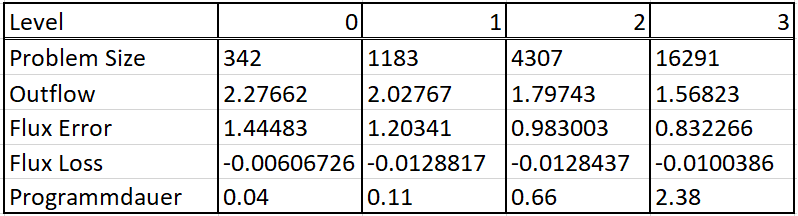
\includegraphics[width=0.99\textwidth]{../Aufgabe35/35_1_linear.png}}	 
\end{figure}

\begin{figure}[H]
	\centering
	\captionabove{Discretization = serendipity}
	\subfigure{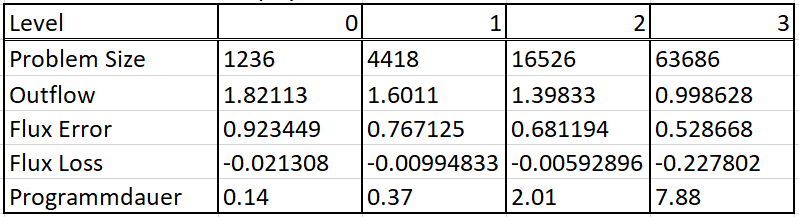
\includegraphics[width=0.99\textwidth]{../Aufgabe35/35_1_serendipity.png}}	 
\end{figure}
Man sieht sehr leicht, dass bei ähnlicher Problemgröße die quadratischen Ansatzelemente den linearen Ansatzelementen überlegen sind. Beispielsweise liefert der lineare Ansatz auf Level 1 (Problemgröße $\approx$ $1200$) einen Flux Error von $\approx 1.2$, während der quadratische Ansatz aus Level 0 (ebenfalls Problemgröße $\approx$ $1200$) mit einem Flux Error von $\approx 0.92$ genauer ausfällt. Diese Erkenntnis zieht sich auch bei anderen Wertepaaren durch die Tabelle.
Wir können dies auch von theoretischer Seite aus erklären:

Sei $V$ der Ansatzraum und $a(\cdot,\cdot)$ die zugehörige Bilinearform unseres aktuell gewählten Verfahrens (Finite Elemente bzw. Discontinuous Galerkin).
Wir erhalten dann im folgenden Lemma eine Aussage über die Güte unserer Approximationslösung:

\begin{Lemma}[Cea's Lemma]
  Sei $a(\cdot,\cdot)$ beschränkt und elliptisch, d.h.
  \begin{align*}
    |a(u,v)| \le C \|u'\| \|v'\|, \quad a(u,v) \ge c \| v'\|^2
    \quad \forall u,v \in V.
  \end{align*}
  Dann gilt für den Galerkin-Fehler $e_h = u-u_h$
  \begin{align*}
    \| e_h' \| \le \frac{C}{c} \inf\limits_{v_h \in V}
    \| u'-v_h' \|.
  \end{align*}
\end{Lemma}
Mit anderen Worten heißt das: Die berechnete Galerkin Approximation ist bezüglich einer geeigneten Norm eine Bestapproximation in unserem Ansatzraum $V$.
Die Vorraussetzungen des obigen Lemmas sind sowohl für die FEM als auch für das DGV erfüllt (vgl. Bericht 1-3 und
Eigenschaften von $ \asip(\cdot,\cdot) $ im ersten Kapitel).
Wir erhalten deshalb für quadratische Ansatzelemente auch eine etwas bessere Lösung, denn der Ansatzraum $V_h^{lin}$ der linearen Ansatzelemente ist natürlich Teilmenge des Ansatzraumes $V_h^{quad}$ der quadratischen Ansatzelemente. Da es sich bei der Finite Elemente Lösung um eine Galerkin-Approximation handelt und diese nach obigem Lemma eine Bestapproximation im zugehörigen Ansatzraum darstellt, kann die Lösung im größeren Ansatzraum $V_h^{quad}$ nur besser ausfallen.

Erstaunlich ist dabei, dass die Programmdauer bei minimal größerer Problemgröße und zudem besserer Genauigkeit bei den quadratischen Ansatzelementen für ungefähr gleiche Problemgröße dennoch meist geringer ausfällt als bei linearen Ansatzelementen. Zum Beispiel liefert Level 2 bei den lineare Ansatzelementen eine Programmdauer von 0.66 Sekunden, bei den quadratischen Ansatzelementen auf Level 1 aber nur von 0.37 Sekunden (Problemgröße $\approx 4350$ bei beiden).



\subsubsection{Aufgabe 35.2}
Als nächstes wollen wir uns dem DG-Ansatz widmen. Wir vergleichen hierbei  \unklar{EINLEITUNG???}

\begin{figure}[H]
	\centering
	\captionabove{symmetric}
	\subfigure{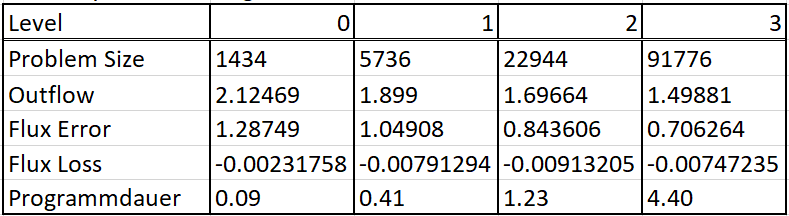
\includegraphics[width=0.99\textwidth]{../Aufgabe35/35_2_sym.png}}	 
\end{figure}


\begin{figure}[H]
	\centering
	\captionabove{non-symmetric}
	\subfigure{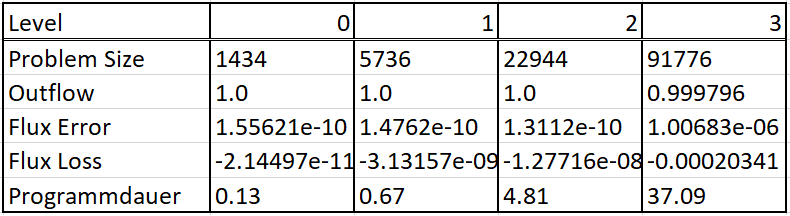
\includegraphics[width=0.99\textwidth]{../Aufgabe35/35_2_nonsym.png}}	 
\end{figure}

Wir wollen nun auf die Vor- und Nachteile bei symmetrischer und nicht-symmetrischer Konfiguration eingehen.
Schnell fällt ins Auge, dass die Ergebnisse des nicht-symmetrischen Verfahrens deutlich besser sind als mit symmetrischer Konfiguration. Während nämlich der Flux Error auf allen Leveln bei der symmetrischen Konfiguration nahe 1 ist, bewegen wir uns bei nicht-symmetrischer Konfiguration im Bereich von (sogar meist besser als) $10^{-6}$. Allerdings sieht man auch sehr schnell ein, dass dies nur auf Kosten der Programmdauer möglich ist. Während auf Level 3 der symmetrische Fall nur 4,4 Sekunden dauert, benötigt das nicht-symmetrische Verfahren sogar fast das 10-fache (ca. 40 Sekunden). 

\subsubsection{Aufgabe 35.3}
\begin{figure}[H]
	\centering
	\captionabove{deg = 2}
	\subfigure{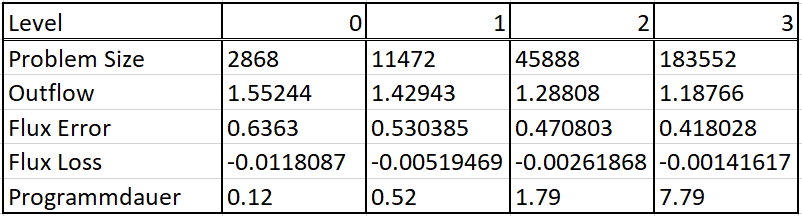
\includegraphics[width=0.99\textwidth]{../Aufgabe35/35_3_level.png}}	 
\end{figure}

Wie bei vorherigen Berichten berechnen wir auch hierzu mithilfe des Flux Errors eine Annäherung an die Konvergenzrate $p$ für den DG Ansatz mit quadratischen Ansatzelementen und symmetrischer Konfiguration.
Wir erhalten 
\begin{align*}
 \frac{e_l^{flux}}{e_{l+1}^{flux}} \approx 1.1508.
\end{align*}
Daraus erhalten wir die Konvergenzrate
\begin{align*}
  p \approx 0.2027.
\end{align*}

\subsubsection*{Penalty}
Wir betrachten nun den Einfluss des Parameters penalty auf das symmetrische DGV mit quadratischen Ansatzelementen.

\begin{figure}[H]
	\centering
	\captionabove{deg = 2, symmetrisch, level = 3}
	\subfigure{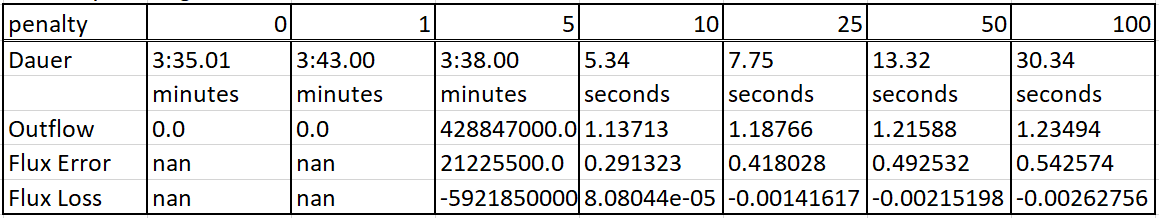
\includegraphics[width=0.99\textwidth]{../Aufgabe35/35_3_dauer.png}}	 
\end{figure}

Wie wir anhand der Tabelle sehen, ist das Verfahren für zu kleinen penalty instabil. Für penalty = 0,1,5 liefert das Verfahren keine brauchbaren Ergebnisse und benötigt eine lange Programmlaufzeit.
Für penalty = 10 erhalten wir eine gute Lösung bei relativ geringer Programmlaufzeit. Erhöhen wir nun den penalty noch weiter, so wird die Programmlaufzeit größer und zugleich die Lösung sogar schlechter. Es gilt also den penalty optimal in der Hinsicht zu wählen, dass das Verfahren stabil ist und der penalty trotzdem möglichst gering.



\subsubsection*{Problemgröße}
Wir wollen uns im Folgenden überlegen, wie die Anzahl der Unbekannten bei den unterschiedlichen Konfigurationen zustande kommen. 
Betrachten wir hierbei zunächst die FEM mit linearen Ansatzelementen stellen wir fest, dass sich die Problemgröße ungefähr in der Größenordnung der Anzahl der Knoten bewegt.
Wir können dies dadurch erklären, dass wir in unserem Ansatzraum für jeden Einzelknoten eine 'Hütchenfunktion' wählen können, welche einen Freiheitsgrad in der Gesamtapproximation ergibt.
Was wir allerdings noch beachten müssen, ist, dass die Dirichletränder bereits fest in unserem Ansatzraum $V_h(0)$ eingebaut sind, weswegen wir Knoten an Dirichleträndern nicht betrachten dürfen.
Es war uns leider nicht möglich die genaue Zusammensetzung der Problemgröße nachzuvollziehen. Was uns verwundert, ist, dass selbst auf verschiedenen Meshes mit gleich vielen Knoten bei gleichem Problem unterschiedliche Problemgrößen zustandekommen:
\begin{itemize}
  \item UnitSquare Lv4 = 289 (=Anzahl der Knoten)
  \item 2Triangles Lv4 = 321
  \item 8Triangles Lv3 = 353
  \item Square500  Lv0 = 342
\end{itemize} 
Sehr schön sieht man allerdings, dass wir pro Level ungefähr eine Vervierfachung der Problemgröße erhalten. Dies ist der Tatsache geschuldet, dass wir durch die Halbierung der Gitterweite viermal so viele Knoten erhalten.

Betrachten wir nun quadratische Ansatzelemente, erhalten wir auf Level 0 im Vergleich zu lineare Ansatzelementen ebenfalls etwa das Vierfache. Auch dies versuchen wir wieder anschaulich zu erklären: 
Wir können uns bei der Überlegung, wieviele Freiheitsgrade hinzukommen, einer einfachen Analogie bedienen: 
Durch die Wahl von quadratischen Ansatzelementen erhalten wir auf jeder Kante, also zwischen zwei Knoten, einen zusätzlichen Freiheitsgrad. Man kann also einsehen \textcolor{green}{??? BILD}, dass wir insgesamt in etwa so viele Freiheitsgrade erhalten, wie bei einem Gitter halber Gitterweite vorliegen. Das heißt wir erhalten beim Schritt von linearen zu quadratischen Ansatzelementen auch wieder ungefähr eine Vervierfachung des Ausgangswertes. Innerhalb der Diskretisierung mit quadratischen Ansatzelementen sehen wir erneut das Verhalten wie zuvor bei den linearen Ansatzelementen, d.h. eine Erhöhung des Levels um 1 hat eine Vervierfachung der Problemgröße zu folge.

\begin{figure}[H]
	\centering
	\captionabove{Problemgröße}
	\subfigure{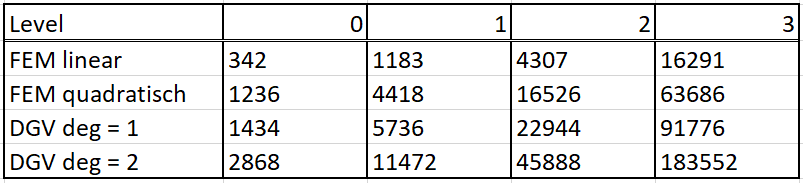
\includegraphics[width=0.99\textwidth]{../Aufgabe35/blub.png}}	 
\end{figure}

Betrachten wir nun das Discontinous Galerkin Verfahren. Wir müssen hierbei beachten, dass wir nun auch unstetige Ansätze erlauben. Es sind also auf den Knoten auch Sprungstellen erlaubt. Wir können uns auch hier einer einfachen Analogie bedienen und betrachten für jeden Knoten für jede anliegende Zelle einen eigenen Hilfsknoten. In unserem Fall erhalten wir bei linearen Ansatzelementen für jede Zelle gerade drei dieser Hilfsknoten (Square500 ist aus Dreiecken aufgebaut). Wir erhalten also für Level 0 (478 Zellen) gerade $3 \cdot 478 = 1434$ Freiheitsgrade. Mit steigendem Level erhalten dann exakt viermal so viele Freiheitsgrade, da bei Halbierung der Gitterweite sich die Zellenanzahl vervierfacht. 

Betrachten wir nun erneut den Schritt von deg = 1 auf deg = 2 können wir die gleiche Analogie wie bereits bei der FEM nutzen. Wir erhalten also bei den quadratischen Ansatzelementen jeweils auf den Kanten einen weiteren Freiheitsgrad. Nun ist aber auch dieser Parameter wieder unstetig wählbar. Mit dem gleichen Trick wie zuvor bei deg = 1 können wir uns also überlegen, dass wir nun auch für jede Kante für jede angrenzende Zelle einen Freiheitsgrad erhalten und so gerade auf das sechsfache der Zellenanzahl kommen (jede Zelle hat 3 Ecken und 3 Kanten).
Auch diese Werte lassen sich genau so in der Tabelle wiederfinden und wir können insgesamt die Verdopplung der Freiheitsgrade beim Schritt von deg = 1 auf deg = 2 feststellen.









\end{document}

